
\documentclass[8pt]{beamer}
\usepackage[authoryear,round]{natbib}
\usepackage{graphicx}
\usepackage{fancybox}
\usetheme[width=2cm]{Goettingen}
\usepackage[utf8x]{inputenc}
\usepackage[T1]{fontenc}
\usepackage[french]{babel}
\usepackage[small]{caption}
%%%Pour Nicolas Bredèche à l'occasion d'une de mes montées à Paris.

\author{Simon Carrignon\\-\\Université Paris 7}
\title{Théorie de l'évolution, principes, histoire et débats actuels}
\begin{document}

\begin{frame}
	\titlepage
\end{frame}
\section{Introduction}
\begin{frame}{Introduction}
	Essayer de comprendre la théorie de l'évolution selon Darwin :
	\vfill
	\begin{itemize}
		\item Fondements théoriques,
		\item histoire et
		\item problèmes.
	\end{itemize}
	\vfill
	Présentation en grande partie reprise des travaux de Gayon 1991.
\end{frame}

\section{La théorie de l'évolution}
\begin{frame}{La théorie darwinienne de l'évolution}
	Chez Darwin:
	\begin{quote}
		Theory of descent with modification by variation and Natural Selection
	\end{quote}

	\vfill

	Deux composantes :
	\begin{itemize}
		\item Descente avec Modification : variation aléatoire et hérédité.
		\item L'Hypothèse de la sélection naturelle : ``survival of the fittest'' (formulation de Spencer).
	\end{itemize}
	\vfil
	Conséquences : une théorie qui explique comment les espèces se modifient \emph{et} se différencient.
\end{frame}

\subsection{Descente avec modifications}
\begin{frame}{Descente avec modifications}
La théorie de l'évolution de Darwin se base sur le fait qu'il y a :
	\begin{itemize}
		\item transmission parents/enfants des caractères, 
		\item des caractères qui varient.
	\end{itemize}
	\vfil
	C'est ce qu'il appelle la \emph{descente avec variation}.
	\vfill 
	\`A l'époque de Darwin : 

\vfil
	\begin{itemize}
		\item Pas de théorie de l'hérédité !
	\end{itemize}
	Hors Darwin admet certaines propriétés aux variations : elles doivent être \emph{aléatoires} et \emph{graduelles} (variant de façon quasi continue). 

\end{frame}

\begin{frame}{Critique de Jenkin}
	Cette caractérisation de la variation engendre de nombreux problèmes que Jenkin va pointer du doigt:
	\begin{beamerboxesrounded}{}
		\begin{itemize}
			\item Si variation admise par Darwin: 
				\begin{itemize}
					\item pas de fixations de nouveaux caractères
					\item pas d'évolution.
				\end{itemize}
			\item critique la plus sérieuse selon Darwin
		\end{itemize}
	\end{beamerboxesrounded}
	\vfill
	Cette critique (très réactionnaire) a le mérite de :
	\begin{itemize}
		\item Proposer les statistiques comme outil d'étude en biologie.
		\item A poussé biologistes à se concentrer sur l'origine des variations (préfigure mendélisme, conflit gradualisme/saltationisme)
	\end{itemize}

\end{frame}


\subsection{Sélection Naturelle}

\begin{frame}{Hypothèse de la Sélection Naturelle}
	Hypothèse : \emph{si} descente avec modification et ressources limitées \emph{alors} :

	\begin{center}
		\emph{Survival of the fittest} (Spencer 1864)
	\end{center}

	Autrement dit, il la \emph{Sélection Naturelle} peut jouer son rôle.
	\vfill
	Problème: hypothèse difficile à prouver (Darwin ne le fera pas).
	\vfil
	Pour l'appuyer Darwin propose:
	\begin{itemize}
		\item Analogie avec la Sélection Artificielle : si SA permet de modifier les races, alors dans la nature SN aussi
	\end{itemize}

	\vfill


	$\rightarrow$ Une théorie de l'évolution solide mais qui manquent de preuves et de support empirique.
\end{frame}
\section{L'après Darwin}
\subsection{Les Biométriciens}
\begin{frame}{Les Biométriciens}
	
\'Ecole initiée par Galton (cousin de Darwin), actifs entre 1890 - 1916 : Pearson, Weldon.
\vfil

Leur but : prouver l'action de la Sélection Naturelle.
	\begin{itemize}
		\item ``Preuve'' mathématique (statistique).
		\item indépendante de théories physiologiques sous-jacentes.
		\item Philosophie très différente.
	\end{itemize}
	\begin{figure}[h]
		\begin{center}
			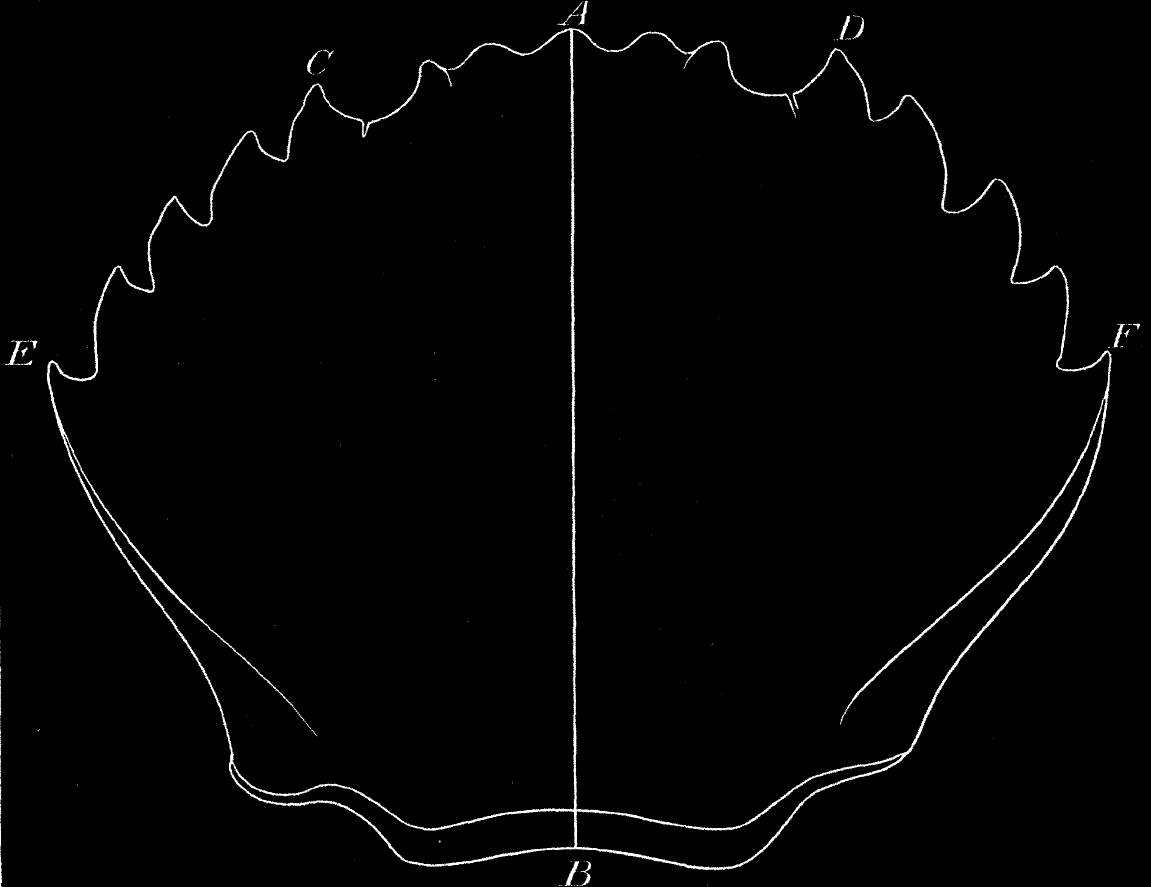
\includegraphics[width=6cm]{images/crabe.png}
		\end{center}
		\label{fig:crabe}
	\end{figure}



\end{frame}

\begin{frame}{}
	\begin{columns}
		\column{.4\textwidth}
	\begin{figure}[hbp]
		\begin{center}
			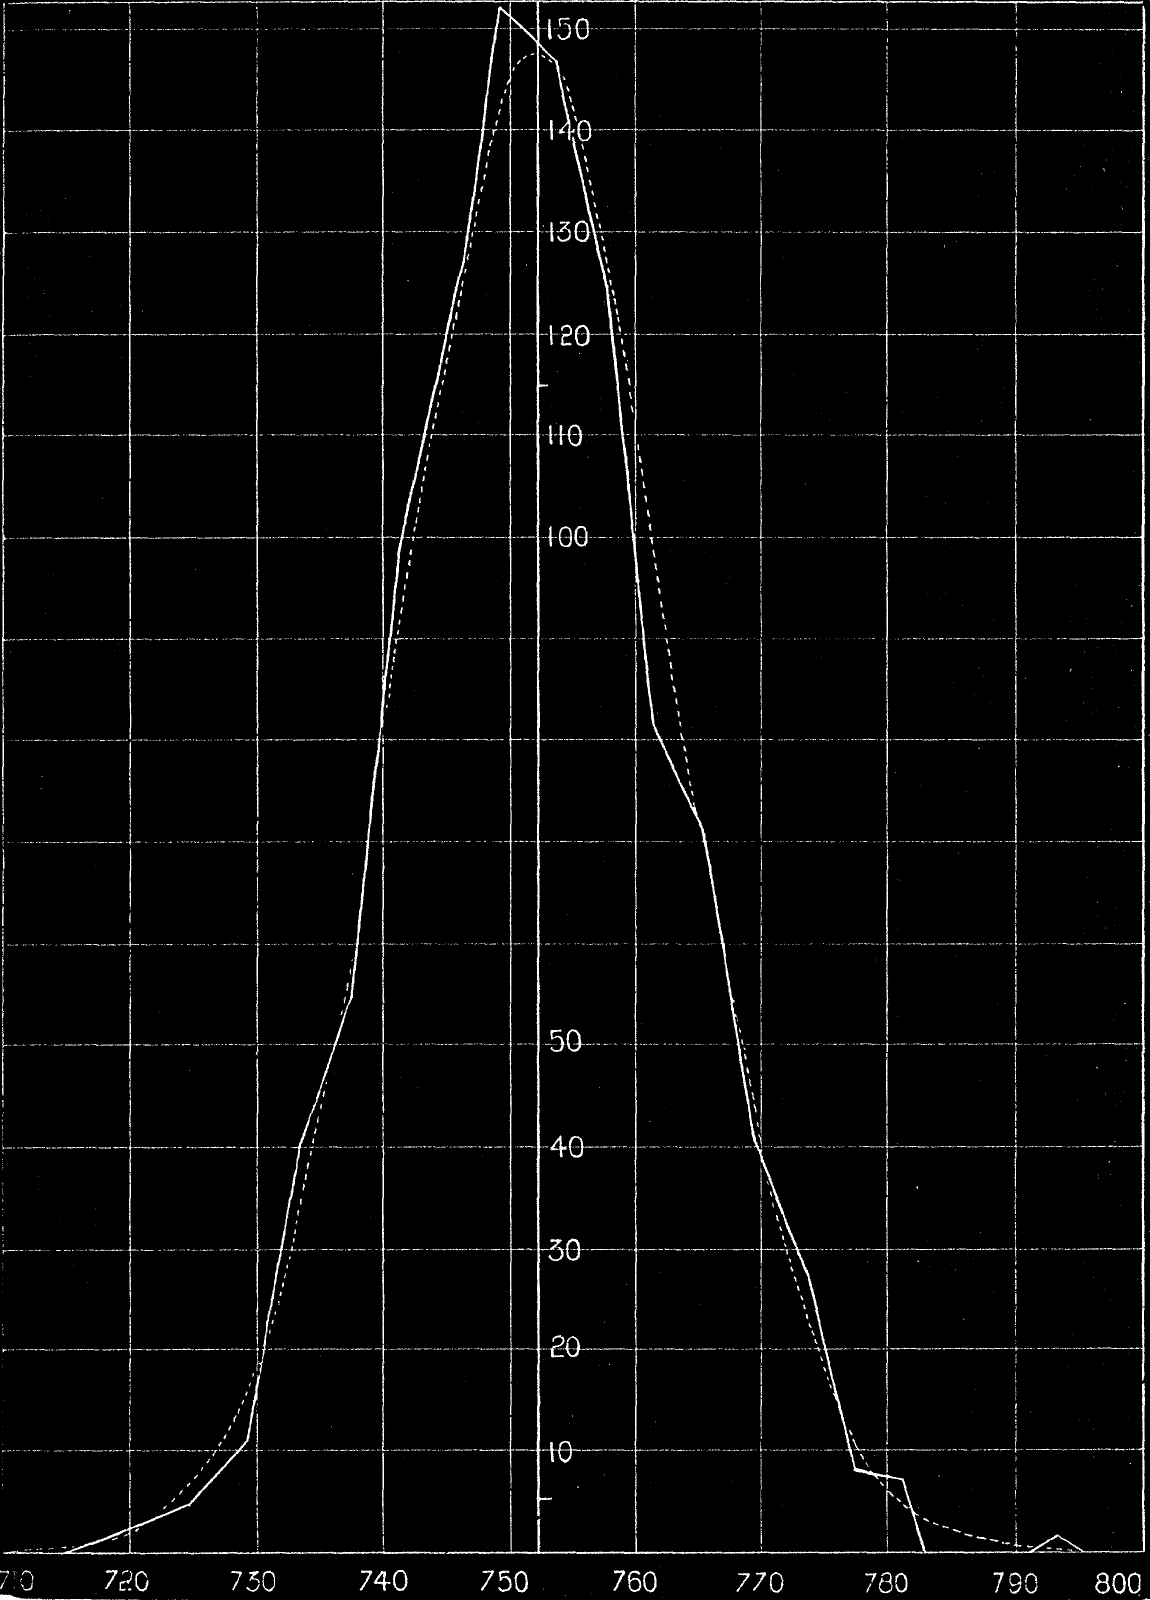
\includegraphics[width=4cm]{images/gauss1.png}
		\end{center}
	\end{figure}

	\column{.6\textwidth}

	\begin{figure}[hbp]
		\begin{center}
			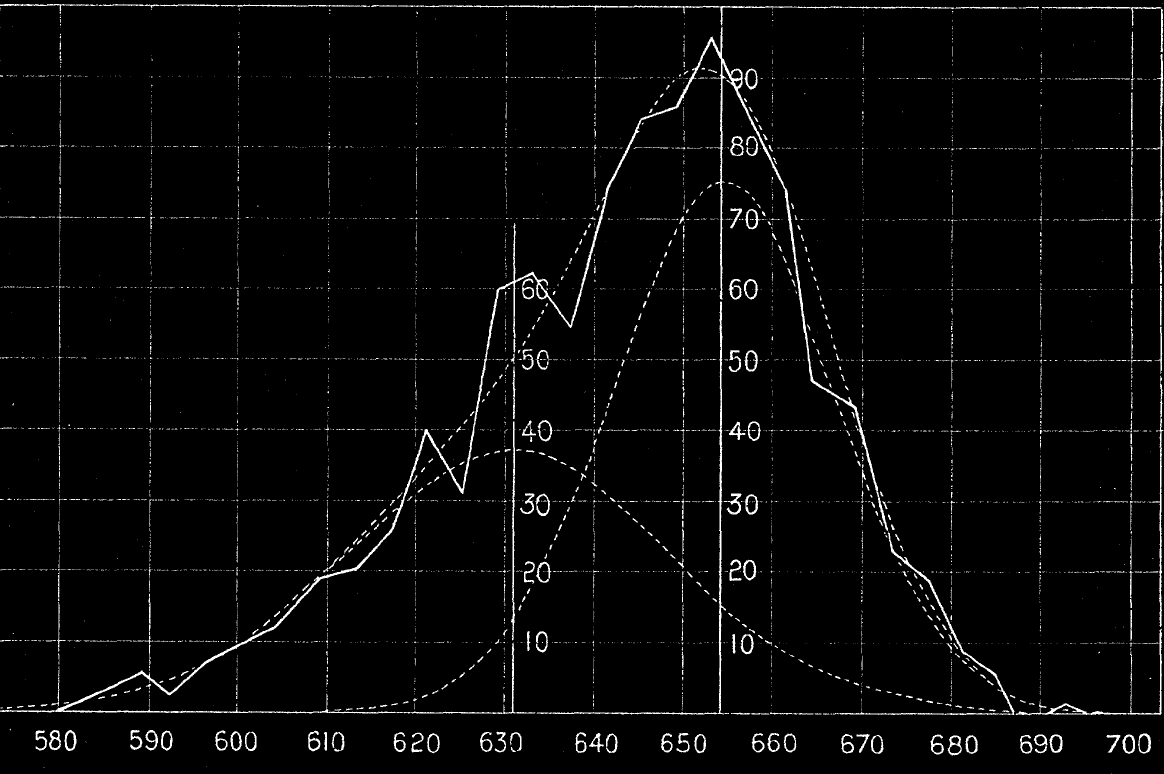
\includegraphics[width=6cm]{images/gauss2.png}
		\end{center}
	\end{figure}
\end{columns}
\begin{center}
	(images extraites de Weldon 1893)
\end{center}

\end{frame}


\subsection{Le mendélisme}
\begin{frame}{Le mendélisme}
	Début du XXe : redécouverte des travaux de Mendel (De Vries):
	\vfill
	\begin{itemize}
		\item pas de variations continues,
		\item caractères atomiques qui s'hybrident
		\item évolution par ``sauts'' (saltationisme) \& ``mutation'' (mutationisme)
	\end{itemize}
	\vfill

	Découvertes en contradiction avec Darwin

	$\rightarrow$ les espèces apparaissent lors de mutation, par ``sauts'' : il n'y a pas de sélection naturelle.

	
\end{frame}



\begin{frame}{Théorie synthétique de l'évolution}
	Réconciliation du mendélisme et de Darwin, la théorie génétique de l'évolution Fisher 1918, avec Haldane et Wright.\\

	$\rightarrow$ invention de la génétique des populations.
	\vfill 

	Visions différentes entre les acteurs :
	\begin{itemize}
		\item Fisher : Idéal Newtonien ``Théorème fondamental de la Sélection Naturel''.
		\item Wright : importance des interactions locales ``Paysages Adaptatifs''.
	\end{itemize}

	\begin{columns}
	\column{.5\textwidth}
		\begin{figure}[hbp]
			\begin{center}
				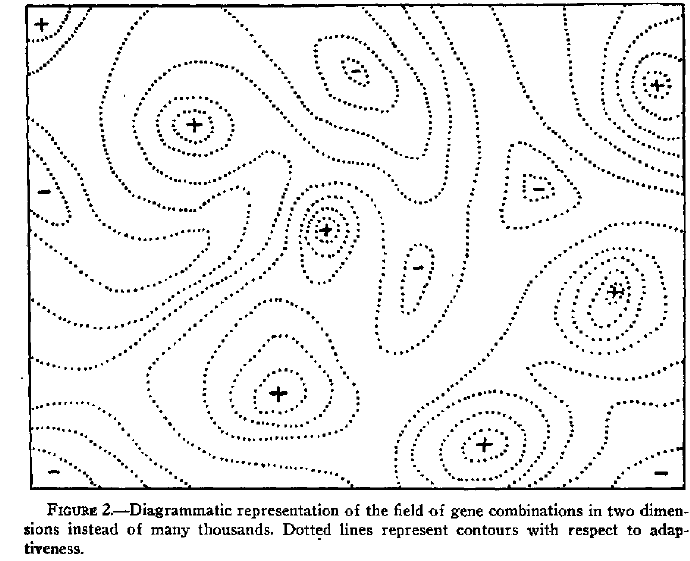
\includegraphics[width=4cm]{images/wrightFL.png}
			\end{center}
		\end{figure}
	\column{.5\textwidth}
		\begin{figure}[hbp]
			\begin{center}
				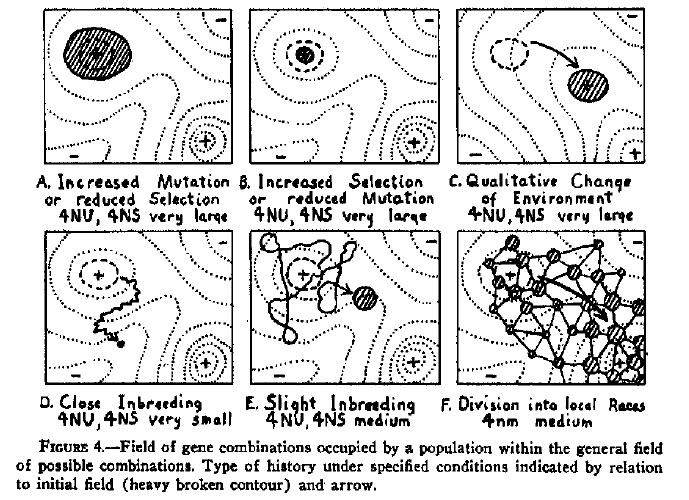
\includegraphics[width=5cm]{images/wrightFL2.png}
			\end{center}
		\end{figure}
	\end{columns}

	\vfill
	Années de synthèses : les différents domaines de la biologie rattachés à la théorie génétique de la Sélection Naturelle. (30's 60's).

\end{frame}

\subsection{Théorie Synthétique de l'\'Evolution}
\begin{frame}{Théorie synthétique de l'évolution}
	Synthèse Moderne :
	\begin{itemize}

		\item	Les individus biologiques sont le produit de l'information génétique transmise par les gamètes (Weismann et dogme central):

			\begin{center}
				ADN$\rightarrow$transcription$\rightarrow$traduction$\rightarrow$protéine
			\end{center}

		\item L'information génétique et transmise de $G^-$ en $G^-$ via l'ADN et varie aléatoirement.

	\item L'évolution correspond à des changements de fréquences alléliques.

	\end{itemize}

	


\end{frame}


\section{Débats actuels}
\subsection{Niveaux et unités de sélection}
\begin{frame}{Niveaux et unités de sélection}

	Définition de l'évolution par Lewontin:
	\vfill
	Dans un population,
	\begin{enumerate}
		\item indiv. $\ne$ $\rightarrow$ morpho., physio., comportements $\ne$ (\alert{variation phénotypique}).
		\item phénotypes $\ne$ $\rightarrow$ des taux de survie et reproduction $\ne$ dans des env. $\ne$ (\alert{fitness différentielle}).
		\item corrélation entre parents et descendants à chaque $G^-$ future (\alert{hérédité de la fitness}).
	\end{enumerate}
	\vfill

	Cette définition n'impose pas un niveau d'orga. biologique. 
	
	Qui, quel niveau d'orga. présente ces propriétés? (gène, chromosomes, organisme, organes, espèces\ldots)?
\end{frame}

\begin{frame}{Niveaux et unités de sélection}
	Après la SM : gène (et donc ADN) est un candidat idéal comme support de l'évolution.
	\vfill
	Les individus sont une $\Sigma$ de gène qui mutent, se croisent et évoluent.
	\begin{itemize}
		\item Dawkin et Williams : \emph{the gene eye view}
	\end{itemize}

	\vfill

	Très vite lacunes pointées du doigts : 
	\begin{itemize}
		\item interactions \emph{many to many}
		\item place grandissante de l'épigénétique
	\end{itemize}
	\vfill

	Peut-on vraiment réduire l'individu et l'évolution au gène? L'étude de l'évolution des gènes peut-elle rendre compte de l'évolution du vivant?
\end{frame}


\begin{frame}{Niveaux et unités de sélection}

	Question complexe avec de multiples approches possible (cf Gould).

	\vfill

	\begin{itemize}
		\item Dichotomie réplicateur/intéracteur-véhicule (Hull-Dawkins) : (Dawkins) les réplicateur sont les gènes et sont sélectionnés et évoluent.
			
			Pdv qui descend de la SM, réductionnisme, \emph{gene eye view} et weismannism.

		\item Superorganisme (Wilson \& Sober) : il y a des niveaux de sélection supérieur différent, on peut expliquer certains phénomène évolutif en étudiant l'évolution à ces niveaux.

		\item \'Ecosystèmes (Bouchard) :  individu est <<\,une entité intégrée fonctionnellement\,>> $\rightarrow$ \'Ecosystèmes, symbioses sont des <<\,individus multi-espèces\,>>. 
			
		Ils présentent <<\,des traits biologiques émergents qu'on ne peut pas réduire à la simple agrégation des phénotypes des individus qui composent ces colonies\,>> sur lesquels la sélection peut agir même si <<\,ces phénotypes ne sont pas ``transmis'' par la seule hérédité génétique\,>> .
	\end{itemize}




\end{frame}

\subsection{Population darwinienne}
\begin{frame}{Godfrey-Smith : population darwiniennes}
	D'après Peter Godfrey-Smith les ``recettes'' posent problème:
	\vfil
	\begin{itemize}
		\item Mixent deux objectifs difficilement conciliables :
			\begin{itemize}
				\item Algorithme ``universel''
				\item Décrire chaque histoire évolutive.
			\end{itemize}
	\end{itemize}
	\vfill
	Pour PGS c'est impossible, il propose en alternative :
	$\rightarrow$ Populations darwiniennes 
	\begin{enumerate}
		\item Minimales (recettes de Lewontin)
		\item Paradigmatiques (multicell. avec reproduction sexuée \ldots )
		\item marginales
	\end{enumerate}

\end{frame}

\begin{frame}{Espace de PGS}
	Partant des propriétés nécessaires aux populations minimales il extrait un ensemble de propriétés:
	\begin{itemize}
		\item H : Fidélité de l'hérédité.
		\item V : Abondance variation.
		\item $\alpha$ : Interaction compétitive vis à vis reproduction.
		\item S : Dépendance de la reproduction différentiée à des facteurs internes.
		\item C : Continuité, régularité du paysage adaptatif.
	\end{itemize}
	\vfil
	
	\begin{figure}[h]
		\begin{center}
			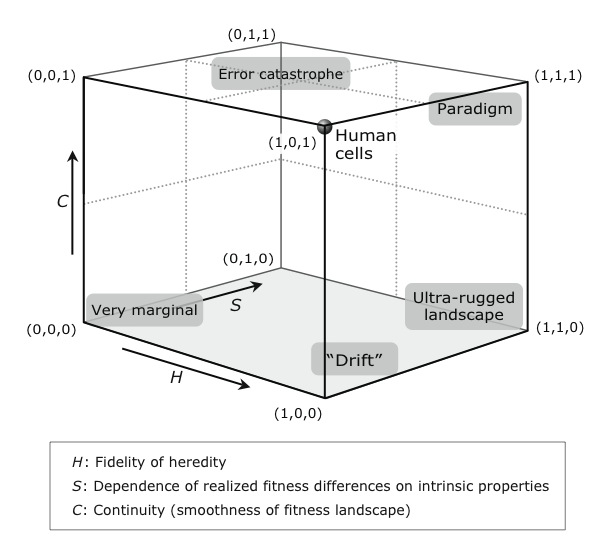
\includegraphics[width=5cm]{./images/PGS.png}
		\end{center}
		\caption{L'espace tridimensionnel extrait de PGS (2009, p.64)}
		\label{fig:PGS}
	\end{figure}
\end{frame}

\section{Conclusion}
	
\begin{frame}{Robotique \'Evlutionnaire et Biologie, un échange à double sens}
	Deux éléments qui doivent échanger en continue:
	\begin{itemize}
		\item concepts fondamentaux et théoriques doivent être discutés pour que les transferts Bio $\rightarrow$ Info soient fructueux.
			\vfill
		\item RE : candidate idéale pour explorer ces théories et fournir des éclairages différents (Robot $\rightarrow$ Bio).
	\end{itemize}
		
\end{frame}


\end{document}
